% Largement inspiré par l'excellent exemple français de présentation de Till Tantau (2004) et Philippe de Sousa (2006) : https://github.com/josephwright/beamer/blob/master/doc/solutions/conference-talks/conference-ornate-20min.fr.tex

\usepackage{lmodern}
\usepackage[french]{babel}
\usepackage[utf8]{inputenc}
\usepackage[T1]{fontenc}

\setbeamertemplate{caption}{\raggedright\insertcaption\par} % Suppression du Figure ou Table préfixé dans les \caption par beamer :  https://tex.stackexchange.com/a/82460

\mode<presentation> {
  \usetheme{default}
  \useinnertheme{circles}
  \useoutertheme[subsections=false]{smoothbars}
  \usecolortheme[rgb={0.9,0,0}]{structure}
}

\AtBeginSection[] {
  \begin{frame}<beamer>{Plan de la soutenance}
    \tableofcontents[currentsection]
  \end{frame}
}

\title{Agrandissement d'un écran mobile par réalité augmentée}
\author{Erwan Normand}
\institute{Soutenance de mémoire de maîtrise}
\date{\frenchdate{2018}{08}{29}}

\newcommand{\twocols}[2]{% Side-By-Side colums
  \begin{columns}%
    \begin{column}{0.5\textwidth}#1\end{column}%
    \begin{column}{0.5\textwidth}#2\end{column}%
  \end{columns}%
}
\newcommand{\captionfigure}[3][1]{%
  \begin{figure}%
    \includegraphics[width=#1\textwidth]{figures/#2}%
    \caption{#3}%
  \end{figure}%
}

\begin{document}

\frame{\maketitle}

\begin{frame}{Plan de la soutenance}
  \tableofcontents
\end{frame}

\section{Problématique} % Chapitre d'introduction
\begin{frame}{La réalité augmentée (RA)}
  \twocols{
    contenu
  }{
    \captionfigure{HoloLens_2}{Application dans le HoloLens.}
  }
\end{frame}

\begin{frame}{Combinaison avec téléphone}
  \twocols{
    contenu
  }{
    \captionfigure{Heun2016}{Application de RA sur un téléphone.}
  }
\end{frame}

\section{Travaux reliés} % Chapitre de revue de littérature
\begin{frame}{Titre}
  contenu
\end{frame}

\section{Concept} % Chapitre du concept
\begin{frame}{Titre}
  \begin{figure}
    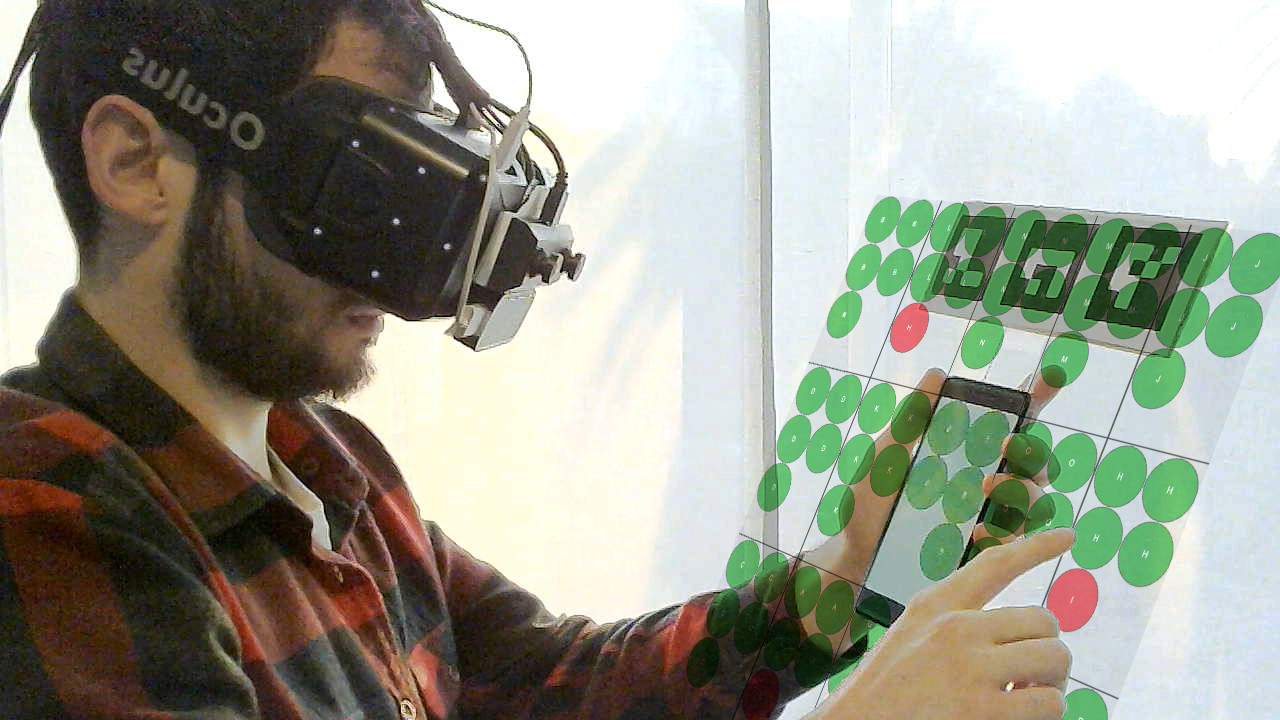
\includegraphics[height=6cm]{figures/HandheldVESADMidAirInArOut}
    \caption{Photomontage de notre prototype.}
  \end{figure}
\end{frame}

\section{Prototype} % Chapitre du visiocasque
\begin{frame}{Titre}
  contenu
\end{frame}

\section{Étude expérimentale} % Chapitre étude expérimentale
\begin{frame}{Titre}
  contenu
\end{frame}

\section{Discussion} % Chapitre discussion
\begin{frame}{Titre}
  contenu
\end{frame}

\section*{Conclusion}
\begin{frame}{Conclusion}
\end{frame}


\appendix
\section<presentation>*{\appendixname}
\begin{frame}{Bibliographie}
\end{frame}

\end{document}